% \tableofcontents
% \newpage

%Definiciónes de comandos y snippets

%SNIPPETS IMPORTANTES:
% gr: pone figuras al 75% de escala
% eq: pone ecuación de linea $$
% mat: matriz de corchetes cuadrados 3x3
% fd: math inline
% ds: display math
%%%%%%%%%%%%%%%%%%%%%%%%%%%%%%%%%%%%%%%
%Comienzo de contenido

\section{Matrices}
\begin{definition}
    El rango de una matriz $A$ de $m \cdot n$ es igual al $min(m, n)$.
\end{definition}
\textbf{Propiedades de la multiplicación:}
\begin{bangenumerate}
    \item $(AB)C = A(BC)$
    \item $A(B+C)= AB + AC$
    \item! $AB \neq BA$, en general
\end{bangenumerate}
\subsection{Operación determinante}
\begin{definition}
    \textbf{Método de los Cofactores:} Sea $A$ una matriz de dimensiones $n \times n$, 
    podemos entonces calcular el determinante de $A$ ($\determinant(A)$ o $|A|$) como sigue.
    Definimos el cofactor de fila $i$ y columna $j$ como:
    \begin{equation*}
        A_{ij} = (-1)^{i+j} \; |M_{ij}|,
    \end{equation*}
    donde $|M_{ij}|$ es el determinante de la matriz $M_{ij}$, que es la matriz de orden $(n-1)\cdot(n-1)$ resultante
    de quitar la i-ésima fila y j-ésima columna de $A$. Luego el determinante de A es la suma de los productos de los
    elemntos de una fila o columna con sus cofactores, es decir.
    \begin{equation*}
        |A| = a_{k1} \cdot A_{k1} + \dots + a_{kn} \cdot A_{kn},
    \end{equation*}
    o también,
    \begin{equation*}
        |A| = a_{1k} \cdot A_{1k} + \dots + a_{nk}\cdot A_{nk}, \; \forall k \in {1, \dots, n}.
    \end{equation*}
\end{definition}

\begin{example}[Filas o columnas de ceros]
    El cálculo de
    \begin{equation*}
        |A| = 
        \begin{vmatrix}
            \sigma & \omega & 0 \\
            \omega & \sigma & 0 \\
            0 & 0 & \lambda \\
        \end{vmatrix},
    \end{equation*}
    se puede realizar rápidamente por método de cofactores, realizando el método en la tercer fila o columna, quedando:
    \begin{equation*}
        |A| = (-1)^{3+3}\lambda \cdot \begin{vmatrix}
            \sigma & \omega \\
            \omega & \sigma \\
        \end{vmatrix} = \lambda \; (\sigma^2 - \omega^2).
    \end{equation*}
\end{example}

\textbf{Propiedades:} Sean A y B matrices cuadradas, entonces

\begin{bangenumerate}
    \item $|A| = |A^t|$,
    \item $|A \cdot B| = |A|\cdot |B|$,
    \item $|A^{-1}| = |A|^{-1}$,
    \item Si $A$ es triangular o diagonal entonces $|A|$ es igual al producto de
    su diagonal principal.
\end{bangenumerate}

\subsection{Operación inversa}
\begin{definition}
    Si $A$ es una matriz no nula de dimensión $n \times n$ entonces
    \begin{equation*}
        A^{-1}  = \frac{Adj(A)^{T}}{|A|},
    \end{equation*}
    donde $Adj(A)$ es la matriz adjunta, es decir aquella que está compuesta por los cofactores de A.
\end{definition}

\textbf{Propiedades:}
\begin{bangenumerate}
    \item $(A^{-1})^{-1} = A$
    \item! $(A\cdot B)^{-1} = B^{-1}\cdot A^{-1}$
    \item $(A^T)^{-1} = (A^{-1})^T$
\end{bangenumerate}

\begin{teorema}
    Una matriz tiene inversa si y sólo si su determinante es distinto
    de cero
    \begin{equation*}
        \exists A^{-1} \Leftrightarrow |A| \neq 0
    \end{equation*}
\end{teorema}


\subsection{Operación Trasposición}
La trasposición de una matriz ($n \times m$), rectangular o cuadrada, es la
reflexión de los elementos respecto de su diagonal principal, adquiriendo
la forma ($m \cdot n$).
\begin{equation*}
    \begin{bmatrix}
        a & b & c \\
        d & e & f \\
    \end{bmatrix}^{T}  =
    \begin{bmatrix}
        a & b \\
        c & d \\
        e & f \\
    \end{bmatrix}
\end{equation*}

\textbf{Propiedades:}
\begin{bangenumerate}
    \item Involutiva: $(A^t)^t = A$
    \item Distributiva: $(A+B)^t = A^t + B^t$
    \item! Producto: $(A \cdot B)^t = B^t \cdot A^t$
\end{bangenumerate}


\newpage
\section{Espacios Vectoriales y Transformaciones Lineales}
\begin{definition}
    Sea $ \bm{X} = \{ \bm{x_1, x_2} ,\dots, \bm{x_n} \}$ un conjunto de 
    vectores que pertenece a un cierto espacio vectorial.
    \begin{equation*}
        \bm{v} = \alpha_1 \cdot \bm{x_1} + \alpha_2 \cdot \bm{x_2} + \dots + \alpha_n \times \bm{x_n}    
    \end{equation*}
    Se dice que $\bm{v}$ es \textit{Combinación Lineal} del conjunto $\bm{X}$.
\end{definition}
\begin{definition}
    Si la única solución a la combinación del vector nulo,
    \begin{equation*}
        \bm{0} = \alpha_1 \cdot \bm{x_1} + \alpha_2 \cdot \bm{x_2} + \dots + \alpha_n \times \bm{x_n} \;,
    \end{equation*}
    es $\alpha_i = 0$, entonces se dice que el conjunto $\bm{X}$ está compuesto
    por vectores \textit{Linealmente Independientes}.\\
    En otras palabras, se dice que un conjunto de vectores son linealmente independientes si ningún vector del conjunto
    puede ser escrito como combinación lineal del resto.
\end{definition}
\begin{obs}
    Por consecuencia
    \begin{equation*}
       \exists \; \alpha_i / \;\; \bm{x_k} = \alpha_1 \cdot \bm{x_1} + \alpha_2 \cdot \bm{x_2} + \dots + \alpha_n \times \bm{x_n}\; , \;\; \bm{x_k} \in X   
    \end{equation*}
    entonces $X$ es un conjunto de vectores \textit{Linealmente Dependientes.}\\
    De esto también se desprende que $\bm{0}$ no puede ser parte de un conjunto
    de vectores linealmente independientes.
\end{obs} 

\begin{definition}
    Sea $S$ un subespacio de $V$, y sea $B = \{ \bm{b_1 b_2} $ \dots $\bm{b_m} \}$.
    Luego B es una \textbf{base de S} si:
    \begin{enumerate}
        \item $\bm{b_1 b_2}$ \dots $\bm{b_m}$ son linealmente independientes.
        \item $\bm{b_1 b_2}$ \dots $\bm{b_m}$ generan al subespacio $S$.
    \end{enumerate}
\end{definition}

\subsection{Transformación Lineal}\label{sec: trafoLineal}
Queremos enconrtar una matriz $A$ que al multiplicarla por las coordenadas de un
vector $\bm{v}$ en la base $B_1$ ([$\bm{v}]_{B1}$) de como resultado el transformado de
dicho vector escrito en base $B_2$. Es decir:
\begin{equation*}
    [T(\bm{v})]_{B2} = \bm{A} \cdot [\bm{v}]_{B1}
\end{equation*}
donde $T: V \rightarrow W$ tal que $B_1$ es base de $V$ y $B_2$ es base de $W$

\begin{teorema}
    Sean $V$ y $W$ espacios vectoriales de dimensión finita. Supongamos $B_1$
    base de $V$ y $B_2$ base de $W$. Existe una \textbf{única} matriz $A \in M_{n\times n}(\mathbb{R})$ tal que:
    \begin{equation}
        \label{eqn: matrizTransformación}
        [T(\bm{v})]_{B2} = \bm{A} \cdot [\bm{v}]_{B1}
    \end{equation}
    donde $A$ se suele notar como [$T]_{B1\rightarrow B2}$
\end{teorema}
Para obtener esta matriz sólamente necesitamos calcular los tranformados
de la base $B_1 = \{ \bm{v_1} \bm{v_2}$ \dots $\bm{v_n}\}$
\begin{equation}
    \bm{A} = [T]_{B1\rightarrow B2} = 
    \begin{bmatrix}
    \uparrow & \uparrow &  & \uparrow\\
    [T(\bm{v_1})]_{B2} & [T(\bm{v_2})]_{B2} & \dots & [T(\bm{v_n})]_{B2}\\
    \downarrow & \downarrow &  & \downarrow\\
    \end{bmatrix}
\end{equation}
Esta matriz toma vectores en base $B_1$ los transforma y devuelve sus coordenadas
en base $B_2$.\\

\begin{teorema}
    Sean $V$ y $W$ espacios vectoriales de dimensión finita. Sean
    $B_1$ y $B_{1'}$ dos bases de V, y $B_2$ y $B_{2'}$ dos bases 
    de W, donde $T: V \rightarrow W$, entonces
    \begin{equation}
        \label{eqn:camino}
        [T]_{B_{1'} \rightarrow B_{2'}} = [B_2]_{B_{2'}} \;
        [T]_{B_{1} \rightarrow B_{2}} \; [B_{1'}]_{B_1} 
    \end{equation}
\end{teorema}


\vspace*{2pt}

Observemos que por lo tanto, si llamo $\bm{\tilde{A}} = [T]_{B_{1'} \rightarrow B_{2'}}$
entonces podemos escribir (\ref*{eqn:camino}) como
\begin{equation}
    \bm{\tilde{A}} = [B_2]_{B_{2'}} \cdot \bm{A} \cdot [B_{1'}]_{B_1} 
\end{equation}

\vspace*{3pt}

\begin{example}
    Sea $T: \mathbb{R}^3 \rightarrow \mathbb{R}^3 / \; \; T(x, y, z) = (x+y, z)$.
    Si $B = \{(1,0,2);(0,2,1);(0,0,3)\}$ es una base de $\mathbb{R}^3$, hallar $[T]_{B \rightarrow C}$ (siendo C la base canonica)
    y $[T( \bm{v})]_C$ siendo $[\bm{v}]_B = [1,2,0]$

    \vspace*{5pt}

    Sabemos que
    \begin{equation*}
        [T]_{B \rightarrow C} = 
        \begin{bmatrix}
            \uparrow & \uparrow &  \uparrow\\
            [T(1,0,2)]_{C} & [T(0,2,1)]_{C} & [T(0,0,3)]_{C}\\
            \downarrow & \downarrow &  \downarrow\\
        \end{bmatrix}
        =
        \begin{bmatrix}
        1 & 2 & 0\\
        2 & 1 & 3\\
        \end{bmatrix}
    \end{equation*} 

    Luego utilizando la matriz hallada podemos obtener el vector transformado en base
    canonica
    \begin{equation*}
        \begin{split}
            [T(\bm{v})]_C = [T]_{B \rightarrow C} \cdot [\bm{v}]_B \\
            [T(\bm{v})]_C = (5, 4) 
        \end{split} 
    \end{equation*}
    que puede ser verificado buscando $T(\bm{v})$.
\end{example}

%%%%%%%%%%%%%%%%%%%%%%%%%%%%%%%%%%%%%%%%%
\subsection{Autovalores y Autovectores}
\begin{definition}
    Para una matriz $ \bm{A} $, un vector no nulo $ \bm{x}$ se dice que 
    es un autovector de $ \bm{A}$ si
    \begin{equation*}
        \bm{A} \cdot \bm{x} = \lambda \bm{x} 
    \end{equation*}
\end{definition}
\begin{obs}
    Si partimos de la definición entonces podemos operar de la siguiente forma
    \begin{equation*}
        \begin{split}
            \bm{0} &= \lambda \bm{x} - \bm{A} \bm{x}\\
            \bm{0} &= (\lambda \bm{I} - \bm{A})\cdot \bm{x}\\
        \end{split}
    \end{equation*}
    y como $\bm{x}$ es no nulo, el sistema tiene una solución no trivial, por lo que
    \begin{equation}
        \label{eqn:autovalores}
        | \lambda \bm{I} - \bm{A} | = 0
    \end{equation}
    donde el determinante se llama \textit{polinomio carácteristico}, y es un polinomio
    mónico de orden $n$. 
\end{obs}

\begin{definition}
    Si $A \in M_n(\mathbb{R})$ entonces:
\end{definition}
\begin{bangenumerate}
    \item! $\lambda$ es autovalor de $A \Leftrightarrow P(\lambda)=  | \lambda \bm{I} - \bm{A} | = 0$
    es decir, los autovalores son las raices del polinomio característico.
    \item! Si $\lambda$ es autovalor de $A \Rightarrow$ las soluciones no nulas
    del sistema homogeneo $(\bm{A}-\lambda \bm{I})\bm{x}=\bm{0}$ son los
    autovectores asociados a $\lambda$
\end{bangenumerate}

\begin{obs}
    Podemos ver de la definición que los autovectores no son únicos, ya que
    si $\bm{x}$ es un autovector, entonces $\alpha\bm{x}$ también lo es.
\end{obs}

\begin{teorema}
    Si $\lambda$ es un autovalor de $A$ entonces $\alpha + \lambda$ es 
    un autovalor de $\alpha I + A$
\end{teorema}

\begin{definition}
    Sea $A$ una matriz de $n \times n$, y $T$ una matriz no singular también
    de $n \times n$, y sea $\tilde{A} = T \; A \; T^{-1} $, entonces $A$ y $\tilde{A}$
    se dicen \textit{matrices semejantes}. Están relacionadas por la matriz de 
    semejanza $T$.
\end{definition}

\begin{teorema}
    Dos matrices semejantes tienen los mismos autovalores
\end{teorema}

\begin{obs}
    Como toda \textit{TL} $T:V\rightarrow V$ tiene asociada una matriz ($[T]_B$),
    las definiciones de autovalores y autovectores también las podemos aplicar a una matriz.
\end{obs}
\vspace*{1pt}

\begin{example}[]
    Sea $B$ una matriz triángular de orden $3\times 3$ genérica, buscar sus
    autovalores y autovectores:
    \vspace*{5pt}
    Si llamamos
    \begin{equation*}
        B = 
        \begin{bmatrix}
        a & b & c\\
        0 & e & f\\
        0 & 0 & i\\
        \end{bmatrix}
    \end{equation*}
    entonces el polinomio característico queda definido por 
    $P(\lambda) = (\lambda - a)\cdot (\lambda - e) \cdot (\lambda - i)$ por lo tanto
    los autovalores de la matriz B son $\{a, e, i\}$.

    Luego podemos obtener los autovectores planteando lo siguiente
    \begin{equation*}
        \begin{split}
            (\bm{B} - \lambda \bm{I}) \bm{x} &= \bm{0} \\
            \begin{bmatrix}
            a-\lambda & b & c\\
            0 & e-\lambda & f\\
            0 & 0 & i-\lambda\\
            \end{bmatrix} \cdot
            \begin{bmatrix}
            x_1\\
            x_2\\
            x_3\\
            \end{bmatrix} &= \bm{0}
        \end{split}
    \end{equation*}
    por lo que obtenemos el siguiente sistema
    \begin{equation}
        \begin{cases}
            (a-\lambda)\cdot x_1 + b\cdot x_2 + c \cdot x_3 &= 0\\
            (e-\lambda)\cdot x_2 + f \cdot x_3 &= 0\\
            (i-\lambda)\cdot x_3 &=0 \\
        \end{cases}
    \end{equation}
    que define al espacio de autovectores asociado al autovalor lambda.

\end{example}

\subsection{Forma Canónica de Jordan}
Sea \( T: V \rightarrow V\), si el polinomio característico de $T$ se factoriza completamente
existe una base donde la transformación lineal viene dada por una matriz de "m bloques" $(m<n)$ con la siguiente forma.
\begin{equation*}
    J = 
    \begin{bmatrix}
    \bm{A_1} & 0 & \cdots & 0\\
    0 & \bm{A_2} & \cdots & 0\\
    0 & 0 & \ddots & 0\\
    0 & 0 & \cdots & \bm{A_m}\\
    \end{bmatrix}
\end{equation*}
donde cada \(\bm{A_k}\) es un \textit{bloque de Jordan}. Estos tienen una dimensión de $m \times m$, 
donde $m$ es la \textit{multiplicidad algebraica} del autovalor asociado.
\begin{equation*}
    \bm{A_k} = 
    \begin{bmatrix}
    \lambda_k & 1 & \cdots & 0 & 0\\
    0 & \lambda_k & 1 & \cdots & 0\\
    \vdots & \vdots & \vdots & \ddots & \vdots\\
    0 & 0 & 0 & \cdots & \lambda_k\\
    \end{bmatrix}
\end{equation*}

luego cada autovector generalizado lo podemos generar con la siguiente regla.
Sea A una matriz genérica de $n \times n$, entonces el i-esimo autovector generalizado puede ser escrito como:
\begin{equation*}
    \begin{cases}
        A \bm{v_1} &= \lambda \bm{v_1} \\
        A \bm{v_i} &= v_{i-1} + \lambda \bm{v_i}, \; \; i>1
    \end{cases}
\end{equation*}
\begin{example}
    Supongamos que se quiere diagonalizar la siguiente matriz
    \begin{equation*}
        A =
        \begin{bmatrix}
        1 & -2 & 1\\
        0 & -1 & 0\\
        -1 & 1 & 3\\
        \end{bmatrix}
    \end{equation*}
    luego su polinomio característico es \( p(\lambda) = (\lambda+1)(\lambda-2)^2 \), es decir sus
    autovalores son -1 y 2. Ahora buscamos los espacios propios asociados a cada autovalor
    \begin{equation*}
        A + I = \begin{bmatrix}
        2 & -2 & 1\\
        0 & 0 & 0\\
        -1 & 1 & 4\\
        \end{bmatrix}
        ~ \begin{bmatrix}
        -1 & 1 & 0\\
        0 & 0 & 1\\
        0 & 0 & 0\\
        \end{bmatrix}
        \rightarrow 
        \begin{cases}
            y &= x \\
            z &= 0 \\
        \end{cases}
    \end{equation*}
    es decir el primer espacio propio es \( E_{\lambda=-1} = \{(x,x,0): x \in \mathbb{R}  \}\).
    \begin{equation*}
        A - 2I = \begin{bmatrix}
        -1 & -2 & 1\\
        0 & -3 & 0\\
        -1 & 1 & 1\\
        \end{bmatrix}
        ~ \begin{bmatrix}
        -1 & 0 & 1\\
        0 & 0 & 0\\
        0 & 0 & 0\\
        \end{bmatrix}
        \rightarrow 
        \begin{cases}
            z &= x \\
            y &= 0 \\
        \end{cases}
    \end{equation*}

    obteniendo el último espacio propio como \( E_{\lambda=2}  = \{(x,0,x): x \in \mathbb{R}  \}\).
    Como vemos el espacio propio de \(\lambda = 2\) tiene una dimensión menor a su multiplicidad algebraica, por lo que 
    no podría ser diagonalizable. Sin embargo Jordan nos proporciona una manera de encontrar una matriz de transformación \(A\) que 
    aunque no es diagonal, cumple la propiedad de ser triangular.

    Para esto Jordan nos dice que debemos encontrar un tercer vector, linealmente independiente a los vectores encontrados
    en los espacios propios. Lo hacemos con la regla ya mencionada, 
    \begin{equation*}
        (A-\lambda I)\bm{v_2} = v_2
        A - 2I = 
        \begin{bmatrix}
        -1 & -2 & 1\\
        0 & -3 & 0\\
        -1 & 1 & 1\\
        \end{bmatrix}
        \begin{bmatrix}
        x \\
        y\\
        z\\
        \end{bmatrix} = 
        \begin{bmatrix}
            1\\
            0\\
            1\\
        \end{bmatrix}
        \rightarrow 
        \begin{cases}
            z &= 1+x \\
            y &= 0 \\
        \end{cases}
        \rightarrow
        \bm{v_2} = [1, 0, 2]
    \end{equation*}
    luego la matriz de similaridad P / $ J = P A P^{-1}$ queda definida como
    \begin{equation*}
        P = \begin{bmatrix}
        1 & 1 & 1\\
        1 & 0 & 0\\
        0 & 1 & 2\\
        \end{bmatrix}%
        , J = \begin{bmatrix}
        -1 & 0 & 0\\
        0 & 2 & 1\\
        0 & 0 & 2\\
        \end{bmatrix}
    \end{equation*}

\end{example}

%%%%%%%%%%%%%%%%%%%%%%%%%%%%%%%%%%%%%%%%%%%%%
\newpage
\section{Espacio de estados y modelos de función transferencia}

\begin{definition}
    Sea un sistema de segundo orden
    \begin{equation*}
        G (s) = \dfrac{\omega_n^2}{s^2 + 2 \xi \omega_n \cdot s + \omega_n ^2}
    \end{equation*}
    se definen las siguientes cantidades:
\end{definition}
\begin{bangenumerate}
    \item! \; \; $0 < \textbf{$\xi$} \leq 1 $: Relación de amortiguamiento
    \item! \; \; $\sigma = \xi \omega_n$ : Parte real del par de polos
    \item \; \; $\omega_d = \omega_n \sqrt{1- \xi ^2}$ : Parte imaginaria del par de polos
    \item \; \; $s_{1,2} = \sigma \pm j \omega_d$ : Par de polos 
\end{bangenumerate}

\vspace*{5pt}
La respuesta temporal al escalón de este sistema es descripto por

%
\noindent
\begin{minipage}{0.4\linewidth}
    \raggedleft
    \begin{equation*}
        y(t) = 1 - \; e^{-\sigma t } \cdot ( \cos{\omega_d t} + \dfrac{\sigma}{\omega_d}\sin{\omega_d t}) 
    \end{equation*}
    \textbf{Reglas para sistemas de 2do O:}
    \begin{bangenumerate}
        \item \; $Ts = \dfrac{4.5}{\sigma}$
        \item \; $ M_p = 100\% \; exp(\dfrac{-\pi \xi}{\sqrt{1-\xi^2}})$
    \end{bangenumerate}
    \vfill
\end{minipage}% <------- USAR PARA TENER MINIPAGES SIDE TO SIDE
\begin{minipage}{0.4\linewidth}
    \raggedright
    \begin{tikzpicture}
        \begin{axis}[
                width=9cm,
                height=6cm,
                axis lines=middle,
                xmin=0, xmax=15,
                ymin=0, ymax=1.5,
                xlabel=$t$,
                ylabel={$y(t)$},
                xlabel style={at=(current axis.right of origin), anchor=west},
                ylabel style={at=(current axis.above origin), anchor=south},
                xtick={},
                xticklabels={},
                every x tick/.style={black},
                ytick={0, 1, 1.3714},
                yticklabels={$0$, $1$, $M_p$},
                every y tick/.style={black}
            ]
            \addplot[black, densely dotted] coordinates{(3.2236,1.3714)} -- (axis cs:0,1.3714);
            \addplot[black, densely dotted] coordinates{(3.2236,1.3714)} -- (axis cs:3.2236,0);
            %
            \addplot[black, dashed] coordinates{(15,1)} -- (axis cs:0,1);
            %
            
            %
            \addplot[smooth, 
                        black,
                        thick,
                        mark=none,
                        domain=0:12.4,
                        samples=100]
            {1-exp(-0.3*x)*(cos(deg(sqrt(1-0.3^2)*x))+0.3/(sqrt(1-0.3^2))*sin(deg(sqrt(1-0.3^2)*x)))};
            %
            \addplot[black, thick] coordinates{(15,0.9872)} -- (axis cs:12.4,0.9872);
            %
            \coordinate (trleft) at (axis cs:0,0);
            \coordinate (trright) at (axis cs:1.96605,0);
            %
            \coordinate (tr1left) at (axis cs:0.4726,0);
            \coordinate (tr1right) at (axis cs:1.79398,0);
            %
            \coordinate (ess1) at (axis cs:14,1.1);
            \coordinate (ess2) at (axis cs:14,1);
            \coordinate (ess3) at (axis cs:14,0.9872);
            \coordinate (ess4) at (axis cs:14,0.8872);
        \end{axis}
    
        \draw [->] (ess1) node [right] {$\Delta$} -- (ess2);
        \draw [<-] (ess3) -- (ess4);
    
    \end{tikzpicture} 
\end{minipage}%

Ahora queremos encontrar un modelo de función transferencia discreta que imite
el modelo de tiempo continuo. Por lo tanto, definimos:
\begin{equation}
    \label{eqn: RtaEscalonDiscreta}
    y[k] = y[kT] = 1 - (\underbrace{e^{-\sigma T}}_{a})^k \; (\cos{k\overbrace{\omega_d T}^{b} + \dfrac{\sigma}{\omega_d}\sin{\omega_d kT}})
\end{equation}

\begin{center}
    \boxed{
        \begin{tabular}{ccc}
            \textbf{Secuencia}&$\longrightarrow $& \textbf{Transformada $\mathcal{Z}$} \\
            $a^k \sin{bk}$ && $\dfrac{az\sin{b}}{z^2-2az\cos{b}+a^2}$ \\
            &&\\
            $a^k \cos{bk}$ && $\dfrac{z(z-a\cos{b})}{z^2-2az\cos{b}+a^2}$ \\            
            \end{tabular}
    }
\end{center}

Donde la transformada buscada es 
\begin{equation*}
    \mathcal{Z} \{y[k]\} = \underbrace{\dfrac{z}{z-1}}_{\text{$\mathcal{Z}\{ u(t)\}$}} \cdot G(z)
\end{equation*}

Luego aplicando Transformada $\mathcal{Z}$ a la ecuación (\ref*{eqn: RtaEscalonDiscreta}) obtenemos
\begin{equation}
    \begin{split}
        \mathcal{Z} \{y(k)\} = Y(z) &= \dfrac{z}{z-1} - z\cdot [\dfrac{\overbrace{z-a\cos(\omega_d T)}^{\text{$\eta_1(z)$}} }{z^2-2e^{-\sigma T}z \cos{\omega_d T}+e^{-2\sigma T}} + \dfrac{\sigma}{\omega_d}\dfrac{\overbrace{a\sin{\omega_d T}}^{\eta_2(z)}}{\Delta(z^2)}] \\
        &= \dfrac{z}{z-1} \underbrace{\dfrac{N(z)}{(z^2-2az\cos{\omega_d T}+a^2 )}}_{\text{$G(z)$}}
    \end{split}
\end{equation}

por lo tanto, los polos del sistema muestreado son
\begin{equation*}
    z^2 - 2az \cos{\omega_d T} + a^2
\end{equation*}

donde
\begin{equation}
    \begin{split}
        z_{1,2} &= a \cos{\omega_d T} \pm ja\sqrt{1-\cos^2{\omega_d T}} \\
        &= (e^{-\sigma T})\cdot (e^{\pm j\omega_d T})\\[10pt]
        |z_{1,2}| &= e^{-\sigma T}
    \end{split}  
\end{equation}
Es decir que la parte real de los polos en el plano "s" controla la magnitud
de los polos en el plano "z".

\begin{example}
    Sea \(G(s)= \dfrac{4}{s^2+3\cdot 2s+4}\), entonces \(\xi = 0.8, \; \omega_n = 2, \; T_s = 4.5/1.6 \simeq 2.8seg, \; M_p = 1.5\% \)
    \\ \\
    $s_{1,2} = -1.6 \pm j1.2$

    Elijamos como periodo $T=0.2$seg, es decir, tendriamos 14 muestras hasta el tiempo de establecimiento $T_s$. \\
    \\ \\
    \(z_{1,2} = e^{s_{1,2} T} = 0.7053 \pm j 0.1726 \) \\ \\


    \begin{figure}[H]
        \centering
        \begin{subfigure}{0.4\textwidth}
            \centering
            \resizebox{\linewidth}{!}{
            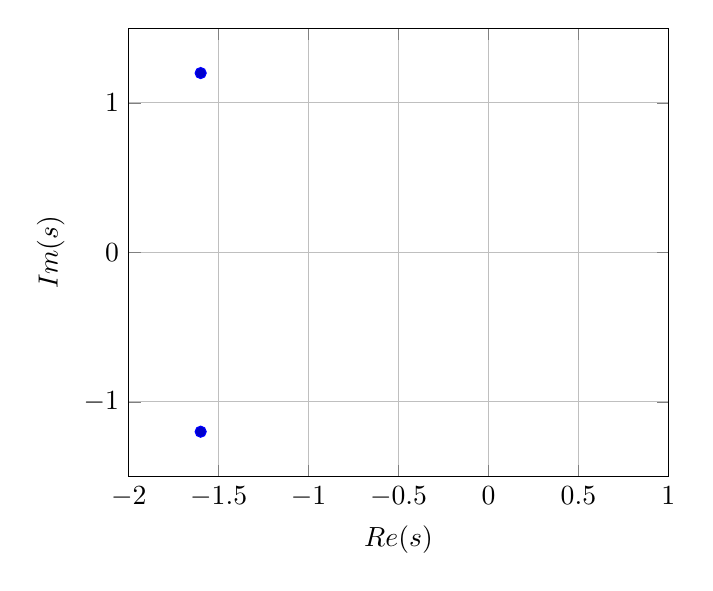
\begin{tikzpicture}
                %\draw[gray, very thin] (0,0) grid (7,5);
                \begin{axis}[
                xmin = -2, xmax=1,
                ymin = -1.5, ymax=1.5,
                grid = both,
                %grid style = {line width = .1pt, draw = gray},
                xlabel={\text{$Re(s)$}},
                ylabel={\text{$Im(s)$}}]
                    %\addplot[domain=0:0.5, color=red] {0};
                    %\addplot[domain=0.6:1,color=red]{0};
                    \addplot+[only marks] coordinates {(-1.6,1.2) (-1.6,-1.2)};
                \end{axis}             
            \end{tikzpicture}
            }
        \end{subfigure}% <---- Importante ese (%) para indicar salto de pag
        \begin{subfigure}{0.4\textwidth}
            \centering
            \resizebox{\linewidth}{!}{
            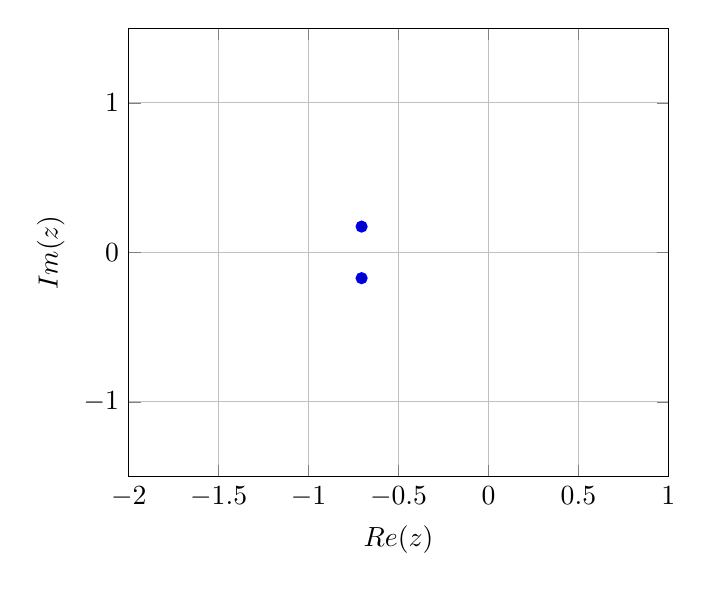
\begin{tikzpicture}
                 \begin{axis}[
                  xmin = -2, xmax=1,
                  ymin = -1.5, ymax=1.5,
                  grid = both,
                  %grid style = {line width = .1pt, draw = gray},
                  xlabel={\text{$Re(z)$}},
                  ylabel={\text{$Im(z)$}}]
                     %\addplot[domain=0:0.5, color=red] {0};
                     %\addplot[domain=0.6:1,color=red]{0};
                     \addplot+[only marks] coordinates {(-0.7053,-0.1726) (-0.7053,0.1726)};
                 \end{axis}             
            \end{tikzpicture}
            }
        \end{subfigure}
    \end{figure}
\end{example}

\subsection{Formas Canónicas}
En esta sección vamos a buscar las matrices de control estándar para una ecuación
diferencial general, que puede contemplar distintos aspectos respecto a su forma de construirse. 
Para esta subsección los resultados están paraemtrizados tanto para sistemas continuos, como para sistemas discretos
con las siguientes ecuaciones diferenciales (o a diferencias): 


\begin{equation*}
    \begin{split}
        \text{\textbf{\underline{Caso continuo:}}} \; \; \boxed{y^{(n)}(t) + a_1 y^{(n-1)}(t) + \cdots + a_n y(t) = b_0 u^{n}(t) + b_1 u^{(n-1)}(t) + \cdots + b_n u(t)}      \\
        \text{\textbf{\underline{Caso discreto:}}} \; \; \boxed{y[k] + a_1 y[k-1] + \cdots + a_n y[k-n] = b_0 u[k] + \cdots + b_n u[k-n]}  \\
    \end{split}
\end{equation*}

Cuyas funciones transferencia son
\begin{equation*}
    \begin{split}
        H(s) = \dfrac{Y(s)}{U(s)} = \dfrac{b_0 s^n + b_1 s^{n-1} + \cdots + b_n}{s^n + a_1 s^{n-1} + \cdots + a_n} \\
        H(z) = \dfrac{Y(z)}{U(z)} = \dfrac{b_0 + b_1 z^{-1} + \cdots + b_n z^{-n}}{1 + a_1 z^{-1} + \cdots + a_n z^{-n}} \\
    \end{split} 
\end{equation*}

En el caso general las ecuaciones de estado se describen como
\begin{equation}
    \text{\underline{Caso Contínuo:}}
    \begin{cases}
        \; \dot{\bm{x}} &= \bm{A} \; \bm{x} + \bm{b} \; u(t) \\
        \; y(t) &= \bm{c} \;\bm{x} + \bm{d} \; u(t) \\
    \end{cases}%
    \hspace*{15pt}
    \text{\underline{Caso Discreto:}}    
    \begin{cases}
        \; \bm{x}[k+1] &= \bm{A} \; \bm{x}[k] + \bm{b} \; u[k] \\
        \; y[k] &= \bm{c} \;\bm{x}[k] + \bm{d} \; u[k] \\
    \end{cases}
\end{equation}
luego podemos plantear las siguientes matrices de estados, llamadas canónicas.
\subsubsection*{Forma Canónica de Observabilidad}
\begin{equation*}
    \bm{A_o} = 
    \begin{bmatrix}
    -a_1 & 1 & 0 & 0 & \cdots & 0\\
    -a_2 & 0 & 1 & 0 & \cdots & 0\\
    -a_3 & 0 & 0 & 1 & \cdots & 0\\
    \vdots & \vdots & \vdots & \vdots & \ddots & \vdots \\
    -a_{n-1} & 0 & 0 & 0 & \cdots & 1\\
    -a_{n} & 0 & 0 & 0 & \cdots & 0 \\
    \end{bmatrix}
    \hspace*{10pt}
    \bm{b_o} = 
    \begin{bmatrix}
    b_1 - a_1\; b_0 \\
    b_2 - a_2\; b_0 \\
    b_3 - a_3\; b_0 \\
    \vdots \\
    b_n - a_n\; b_0 \\
    \end{bmatrix}
    \hspace*{5pt}
    \bm{c:o} = 
    \begin{bmatrix}
    1 & 0 & \cdots & 0
    \end{bmatrix}
    \hspace*{5pt}
    \bm{d_o} = b_0
\end{equation*}


\subsubsection*{Forma Canónica de Controlabilidad}
\begin{equation*}
    \bm{A_c} = 
    \begin{bmatrix}
    -a_1 & -a_2 & -a_3 & \cdots & -a_{n-1} & -a_n\\
    1 & 0 & 1 & 0 & \cdots & 0\\
    0 & 1 & 0 & 1 & \cdots & 0\\
    \vdots & \vdots & \ddots & \vdots & \vdots & \vdots \\
    0 & 0 & 0 & 1 & 0 & 0\\
    0 & 0 & 0 & \cdots & 1 & 0 \\
    \end{bmatrix}
    \hspace*{10pt}
    \bm{b_c} = 
    \begin{bmatrix}
    1 \\
    0 \\
    0 \\
    \vdots \\
    0\\
    \end{bmatrix}
    \hspace*{5pt}
    \bm{c_c} = 
    \begin{bmatrix}
    b_1 - a_1\; b_0 & b_2 - a_2\; b_0 & \cdots & b_n - a_n\; b_0
    \end{bmatrix}
    \hspace*{5pt}
    \bm{d_c} = b_0
\end{equation*}


\begin{example}
    Podemos escribir la función transferencia discreta,
    \begin{equation*}
        H(z) = \dfrac{2 z + 4 z + 4}{z^2 + 2 z},
    \end{equation*}
    observando que \( b_0 = 2, b_1, b_2 = 4, a_1=2, a_2=0\). Por lo tanto,
    \begin{equation*}
        \bm{\dot{x}}[k+1] = 
        \begin{bmatrix}
        -2 & 1\\
        0 & 0\\
        \end{bmatrix}
        \bm{x} +
        \begin{bmatrix}
        0 \\
        4 \\
        \end{bmatrix}
        u[k]
    \end{equation*}
    \begin{equation*}
        y[k] = \begin{bmatrix}
        1 & 0 \\
        \end{bmatrix}
        \bm{x}[k]
        + 2 u[k]
    \end{equation*}
\end{example}

\subsection{Transformaciones de Canon}
Si aplicamos la teoría de la sección () entonces podemos transformar
las matrices de control planteando
\begin{equation*}
    \bm{\bar{x}} = \bm{T} \bm{x} \; \; \text{o también} \; \;\bm{x} = \bm{T^{-1}} \bm{\bar{x}}
\end{equation*}
desde donde podemos demostrar que
\begin{equation*}
    \begin{split}
        \bm{\bar{A}} &= \bm{T} \bm{A} \bm{T^{-1}} \\
        \bm{\bar{b}} &= \bm{T} \bm{b} \\
        \bm{\bar{c}} &= \bm{c} \bm{T^{-1}} \\
        \bar{b} &= b
    \end{split}
\end{equation*}

\subsection{Condiciones Iniciales}
Queremos aproximar al vector de condiciones iniciales, es decir, queremos
conocer el valor de cada variable de estado en un inicio del sistema.
Para esto volvamos al sistema,
\begin{equation*}
    \begin{cases}
        \; \dot{\bm{x}} &= \bm{A} \; \bm{x} + \bm{b} \; u(t) \\
        \; y(t) &= \bm{c} \;\bm{x} + \bm{d} \; u(t) \\
    \end{cases}%
\end{equation*}
suponiendo que \( u^{k}(0^{-})=0 \) entonces podemos plantear que,
\begin{equation*}
    \begin{split}
        y(0^{-}) &= \bm{c} \bm{x}(0^{-}) + d u(0^{-}) = \bm{c} \bm{x}(0^{-}) \\
        y^{(1)}(0^{-}) &= \bm{c} \bm{x^{(1)}}(0^{-}) + d u^{(1)}(0^{-}) = \bm{c} \bm{x^{(1)}}(0^{-}) \\
        y^{(2)}(0^{-}) &= \bm{c} \bm{A} \bm{x^{(2)}}(0^{-}) + d u^{(2)}(0^{-}) = \bm{c} \bm{A} \bm{x^{(2)}}(0^{-}) \\
        \vdots &= \vdots \\
        y^{(n-1)}(0^{-}) &= \bm{c} \bm{A} \bm{x^{(n-2)}}(0^{-}) + d u^{(n-1)}(0^{-}) = \bm{c} \bm{A} \bm{x^{(n-1)}}(0^{-}) \\
    \end{split}
\end{equation*}












